%% 
%% Copyright 2019-2021 Elsevier Ltd
%% 
%% This file is part of the 'CAS Bundle'.
%% --------------------------------------
%% 
%% It may be distributed under the conditions of the LaTeX Project Public
%% License, either version 1.2 of this license or (at your option) any
%% later version.  The latest version of this license is in
%%    http://www.latex-project.org/lppl.txt
%% and version 1.2 or later is part of all distributions of LaTeX
%% version 1999/12/01 or later.
%% 
%% The list of all files belonging to the 'CAS Bundle' is
%% given in the file `manifest.txt'.
%% 
%% Template article for cas-dc documentclass for 
%% double column output.

\documentclass[a4paper,fleqn]{cas-dc}

% If the frontmatter runs over more than one page
% use the longmktitle option.

%\documentclass[a4paper,fleqn,longmktitle]{cas-dc}

% \usepackage[numbers]{natbib}
\usepackage[authoryear]{natbib}
% \usepackage[authoryear,longnamesfirst]{natbib}

\usepackage{hyperref}
\hypersetup{
    % colorlinks = false, % default value = true; used during formatting
    % allcolors = {teal}, % color used while writing, recommanded if within guidelines
    allcolors = {black}, % consistent look
}
\usepackage{cleveref}

%%%Author macros
\def\tsc#1{\csdef{#1}{\textsc{\lowercase{#1}}\xspace}}
\tsc{WGM}
\tsc{QE}
%%%

% Uncomment and use as if needed
%\newtheorem{theorem}{Theorem}
%\newtheorem{lemma}[theorem]{Lemma}
%\newdefinition{rmk}{Remark}
%\newproof{pf}{Proof}
%\newproof{pot}{Proof of Theorem \ref{thm}}


\begin{document}
\let\WriteBookmarks\relax
\def\floatpagepagefraction{1}
\def\textpagefraction{.001}

% Short title
% \shorttitle{<short title of the paper for running head>}    
\shorttitle{Automated machine learning selection system for general prediction}

% Short author
% \shortauthors{<short author list for running head>}  
\shortauthors{Ketkar Y., Gawade S.}

% Main title of the paper
\title [mode = title]{Automated machine learning selection system for general prediction}

\let\printorcid\relax

% Title footnote mark
% eg: \tnotemark[1]
% \tnotemark[<tnote number>] 

% Title footnote 1.
% eg: \tnotetext[1]{Title footnote text}
% \tnotetext[<tnote number>]{<tnote text>} 

% First author
%
% Options: Use if required
% eg: \author[1,3]{Author Name}[type=editor,
%       style=chinese,
%       auid=000,
%       bioid=1,
%       prefix=Sir,
%       orcid=0000-0000-0000-0000,
%       facebook=<facebook id>,
%       twitter=<twitter id>,
%       linkedin=<linkedin id>,
%       gplus=<gplus id>]

\author[1]{Yashodhan Ketkar}

% Corresponding author indication
% \cormark[<corr mark no>]

% Footnote of the first author
% \fnmark[<footnote mark no>]

% Email id of the first author
\ead{ketkaryapr19me@student.mes.ac.in}

% URL of the first author
% \ead[url]{<URL>}

% Credit authorship
% eg: \credit{Conceptualization of this study, Methodology, Software}
% \credit{<Credit authorship details>}

% Address/affiliation
\affiliation[1]{organization={Department of Information Technology Engineering, Pillai College of Engineering},
            % addressline={}, 
            city={New Panvel},
%          citysep={}, % Uncomment if no comma needed between city and postcode
            postcode={410206},
            % state={Maharashtra},
            country={India}}

\author[2]{Sushopti Gawade}

% Footnote of the second author
% \fnmark[2]

% Email id of the second author
\ead{sgawade@mes.ac.in}

% URL of the second author
% \ead[url]{}

% Credit authorship
% \credit{}

% Address/affiliation
\affiliation[2]{organization={Department of Computer Engineering, Pillai College of Engineering},
            % addressline={}, 
            city={New Panvel},
%          citysep={}, % Uncomment if no comma needed between city and postcode
            postcode={410206},
            % state={Maharashtra},
            country={India}}

% Corresponding author text
% \cortext[2]{Corresponding author}

% Footnote text
% \fntext[1]{}

% For a title note without a number/mark
%\nonumnote{}

% Here goes the abstract
\begin{abstract}
    The use of machine learning in various fields is still limited. The driving reason behind this is the lack of ease-to-use systems for non-technical people. The objective of this paper is to provide the general population access to a machine learning system. We propose an automated machine learning system for non-technical users. The proposed system automates the selection of the best model as per user requirements. We employed the proposed system on 3 different datasets in this study. The proposed system showed high accuracy in training the machine learning models and the selection of appropriate models as per user demand. The system showed improvement in performance with a larger data size. As per tests conducted the proposed system showed satisfactory performance.
\end{abstract}

% Use if graphical abstract is present
%\begin{graphicalabstract}
%\includegraphics{}
%\end{graphicalabstract}

% Research highlights
% \begin{highlights}
% \item a
% \item a
% \item a
% \end{highlights}

% Keywords
% Each keyword is seperated by \sep
\begin{keywords}
    Automated Selection System \sep
    General Prediction \sep
    Machine Learning \sep
    Machine Learning in Medical Field \sep
    Supervised Learning Algorithm
\end{keywords}

% \tolerance 9999
% \hbadness=10000

\maketitle


% Main text
% \section{Introduction}\label{sec:introduction}
\section{Introduction}\label{sec:introduciton}

In recent years, machine learning has become very popular. Earlier, machine learning was limited to the research field. But quite recently, it has been used in various fields. This is partially due to the increasing availability of computers and growth in computing power.

The researchers are using machine learning in various fields. One of such fields is solar energy production. In this field, the prediction of solar radiation available per day can be very significant. \cite*{ref_paper_7} employed a few machine learning algorithms for the prediction of the amount of solar radiation received in a day. \citeauthor{ref_paper_7} used natural properties such as weather, time, etc as features for the machine learning algorithms. \citeauthor{ref_paper_7} concluded that supervised learning models gave satisfactory results in predicting the amount of solar radiation. \citeauthor{ref_paper_7} concluded that the ANN model showed great potential for such specialized tasks.

In the field of chemistry, there is a wide range of factors that need to be considered. \cite*{ref_paper_10} used machine learning in the field of chemistry. \citeauthor{ref_paper_10} suggest that the models performed better than conventional statistical methods. \citeauthor{ref_paper_10} concluded that more research is necessary before implementation.

Machine learning can be applied in network security for intrusion detection. \cite*{ref_paper_21} state that the supervised learning methods perform satisfactorily for intrusion detection. \citeauthor{ref_paper_21} also remark that the supervised learning methods are limited to conventional problems.

\cite*{ref_paper_36} in thier study used machine learning models to solve real-life problems. \citeauthor{ref_paper_36} concluded that machine learning plays an important role in good decision-making. \citeauthor{ref_paper_36} also remark that machine learning can be used in various fields.

\cite*{ref_paper_24} note a lack of information and meaningful research in the medical field. \citeauthor{ref_paper_24} suggest that more support, subject-specific scope, and accuracy are important factors for the higher impact of machine learning in the medical field. \citeauthor{ref_paper_24} also suggest that the ideal system should be able to take multiple data types for training.

\cite*{ref_paper_29} used machine learning with a combination of IoT for smart cities. \citeauthor{ref_paper_29} concludes that machine learning showed promising results for smart cities. \citeauthor{ref_paper_29} remark that machine learning was able to handle the high volume of data generated by sensors. \cite*{ref_paper_12} in thier paper suggests that machine learning can handle downstream tasks efficiently.

This suggests that even with the immense popularity and accessibility of machine learning, it is still underutilized by the general population. This can be attributed to lack of knowledge and skills. To solve this problem we are proposing a system with minimum user interaction. The proposed system can be operated by users without prior knowledge of machine learning. This system allows them to train their machine learning algorithms.

The proposed system can be deployed on a local network. The system can feed data manually or automatically according to user needs and policies. The local deployment also limits external access and reduces the influence of external factors on data.

\section{Literature Review}\label{sec:literature_review}

Supervised learning algorithms are widely used in various fields. \cite*{ref_paper_14} conducted a study on the application of machine learning in various industries. \citeauthor{ref_paper_14} suggests that various industries already use supervised learning algorithms to solve various problems. \cite*{ref_paper_6} used machine learning in Civil Structural Health Monitoring (SHM). \citeauthor{ref_paper_6} used supervised learning methods due to the abundance of well-labeled data. \citeauthor{ref_paper_6} concluded that machine learning showed satisfactory results.

Supervised learning algorithms are very efficient in conventional problems. \cite*{ref_paper_9} used machine learning to detect the DDOS attack. \citeauthor{ref_paper_9} used five main security factors as features. \citeauthor{ref_paper_9} conclude that the random forest algorithm was able to detect intrusion with high accuracy.

\cite*{ref_paper_2} conducted a study on the automated selection of SVM algorithms. The goal of the study was to select the most optimal SVM model for a given task. \citeauthor{ref_paper_2} suggested that hyperparameters and used data have an extreme impact on prediction time.

\cite*{ref_paper_38} used machine learning to detect arrhythmia. \citeauthor{ref_paper_38} concluded that SVM achieved up to 91.2\% accuracy. \cite*{ref_paper_16} also used machine learning to detect arrhythmia. The neural network provided good results.

Recently machine learning was used in the diagnosis of COVID-19 disease and study related to its structure. \cite*{ref_paper_20} surveyed the research conducted on the machine learning approach to diagnose the COVID-19. \citeauthor{ref_paper_20} suggested that the supervised learning algorithms showed promising results in diagnosis. \citeauthor{ref_paper_20} suggested that various types of datasets were used in these studies.

Machine learning is used in the diagnosis process. \cite*{ref_paper_34} machine learning is used for the detection of Parkinson's disease. The machine learning algorithm achieved 100\% accuracy with a 95-99\% confidence level. The RF and SVM showed better performance compared to other algorithms. In their paper \cite*{ref_paper_15} suggest that the inclusion of machine learning in diagnosis can lead to better results and higher accuracy. \citeauthor{ref_paper_15} mentions that machine learning can handle a high volume of data.

\cite*{ref_paper_27} reviewed 200 studies published about the use of machine learning in Parkinson's disease diagnosis. \citeauthor{ref_paper_27} found out that the use of machine learning improved clinical decisions. In thier study \cite*{ref_paper_30} used machine learning for the detection of Parkinson's disease. The SVM model outperformed other models. \citeauthor{ref_paper_30} concludes that machine learning provides a better detection method.

Arrhythmias are a symptom of cardiological disorders. \cite*{ref_paper_28} used a supervised learning method for the detection of arrhythmia. The machine learning system provided satisfactory results. Results showed high accuracy and sensitivity. \citeauthor{ref_paper_28} remark on the need for good feature selection and selection guidelines for better-performing algorithms.

The machine learning system needs to be robust, extremely accurate, and easy to use. In the field of healthcare, according to \cite*{ref_paper_4} these are essential requirements. In this study, \citeauthor{ref_paper_4} used machine learning to classify arrhythmia. \citeauthor{ref_paper_4} remark that early detection of arrhythmia is critical for better treatment.

\cite*{ref_paper_32} conducted a study on the automatic selection of machine learning algorithms and their hyperparameters. \citeauthor{ref_paper_32} showed limitations in the biomedical industry with the help of machine learning systems. \cite*{ref_paper_37} studied the security and privacy aspect of machine learning solutions. \citeauthor{ref_paper_37} suggest that while machine learning has great potential in the healthcare system, more research about security and privacy aspects is necessary.

Machine learning utilizes various approaches for the same problem. In thier study \cite*{ref_paper_8} used two approaches to solve a diagnosis problem. In a direct approach, data was fed to a machine learning model. In an indirect approach, data was equalized before the machine learning process. The indirect method showed better results compared to the direct method. While the experiment was successful, \citeauthor{ref_paper_8} suggests that machine learning is still unstable for the medical field.

The supervised learning methods are very effective in the medical field. \cite*{ref_paper_11} suggest that ensembled supervised learning systems can further improve effectiveness. \citeauthor{ref_paper_11} further remark that machine learning will reduce the number of errors caused by humans.

In the review about the use of machine learning in the medical field, \cite*{ref_paper_33} suggested that big companies are already using machine learning for various tasks. \citeauthor{ref_paper_33} suggested that a machine learning system needs to be handled by non-technical people and it should support various ranges and types of data.

The automated system will allow non-technical people to use machine learning. \cite*{ref_paper_3} studied the automatic model selection for optimal SVM kernels. \citeauthor{ref_paper_3} used different automation approaches for optimal hyperparameter calculations. \citeauthor{ref_paper_3} state that the system can calculate up to two parameters without human interaction.

The automatic selection process can be extremely beneficial in dynamic environments. The excavation of soil or tunneling is one such environment. To predict the displacement induced by excavation, \cite*{ref_paper_1} used machine learning. \citeauthor{ref_paper_1} used properties of soli and imputed them as features. \citeauthor{ref_paper_1} concluded that the unsupervised machine learning algorithm GA-MLP showed good potential, while AutoML is found to be the most optimal algorithm in these dynamic conditions. \cite*{ref_paper_13} also suggested that machine learning can be used in dynamic environments successfully.

There are multiple ways to select the best-suited model, the important part of such a system is the selection system. The system uses various approaches for selection, ranking is one of those approaches. In thier study \cite*{ref_paper_23} suggest that the meta ranking is better than the baseline ranking system. \citeauthor{ref_paper_23} used a multi-criteria ranking system for the selection of ideal classifiers. \citeauthor{ref_paper_23} suggest that this study laid some groundwork for future automated machine learning selection systems.

\section{Design and Implmentation}\label{sec:design_and_implmentation}

\subsection{System Architecture}\label{subsec:system_architecture}

The goal of the system is to be used by non-technical users. The system consists of three processes or modules. These processes are the training process, selection process, and prediction process. The first two processes interact with each other. Their task is to produce the best-suited model for the user's needs. The third process interacts with the selected models to generate the predictions. \autoref{fig:system_architecture}, shows the architecture of the system. The user is indirectly allowed to access the training and prediction process. The user data is stored on a local drive for easier and faster access.

\begin{figure}[ht]
    \centering
    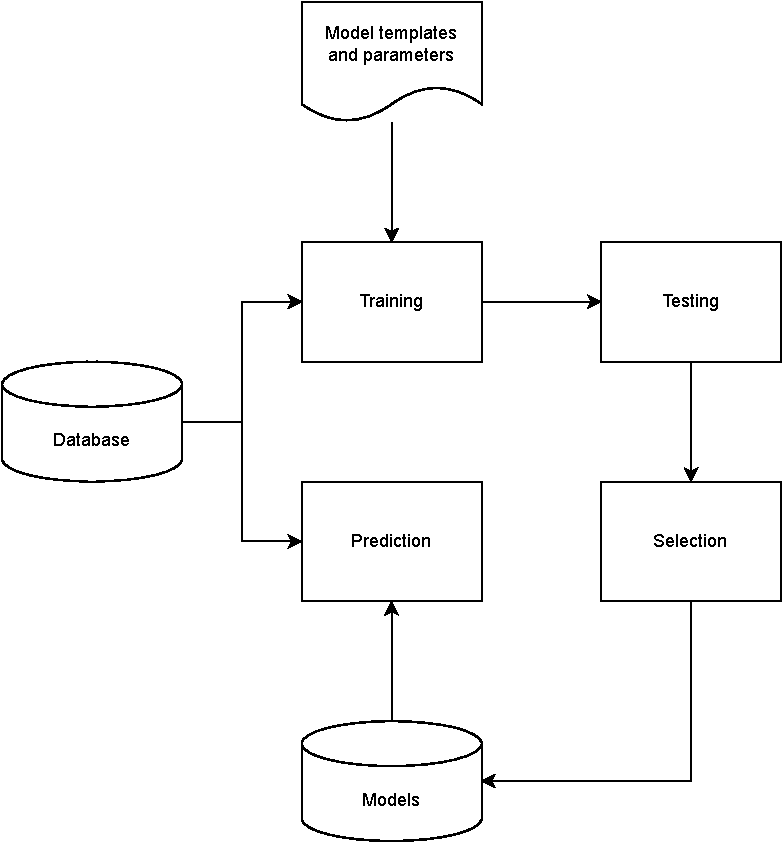
\includegraphics[width=0.9\columnwidth]{media/sec03/system_architecture.pdf}
    \caption{System Architecture}
    \label{fig:system_architecture}
\end{figure}

\subsection{System Processes}\label{subsec:system_processes}

As stated in previous section, the system consists of three primary processes. These processes are the training process, selection process, and prediction process. These processes are described in the following sections.

\subsubsection{Training Process}\label{subsubsec:training_process}

The training process is the first process in the system. \autoref{fig:training_process}, shows the structure of the training process. The training process has many functions. The first function is gathering data from the user and pre-processing it for training purposes. The training process also generates models with the template, which contains model structure and parameters. These models are trained with processed data and stored for future use. The performance of models is also calculated during this phase and store for selection purpose.

\begin{figure}[ht]
    \centering
    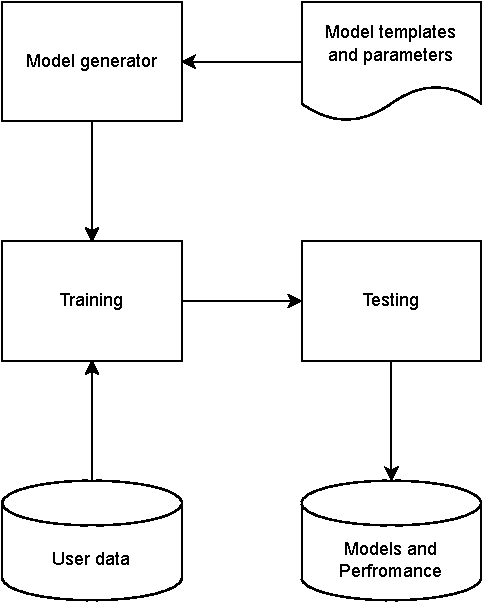
\includegraphics[width=0.6\columnwidth]{media/sec03/training_and_testing.pdf}
    \caption{Training Process}
    \label{fig:training_process}
\end{figure}

\subsubsection{Selection Process}\label{subsubsec:selection_process}

The selection process is second in the system. \autoref{fig:selection_process}, shows the structure of the training process. This process evaluates the performance of models based on metrics and weightage. The metrics of models are generated during the training process. The performance weightage is defined by the user depending on requirements. The final performance score is calculated and used for selection of the best model for users task. The selected model is stored in a separate directory with a label for easier access. This model will be used for prediction problems.

\begin{figure}[ht]
    \centering
    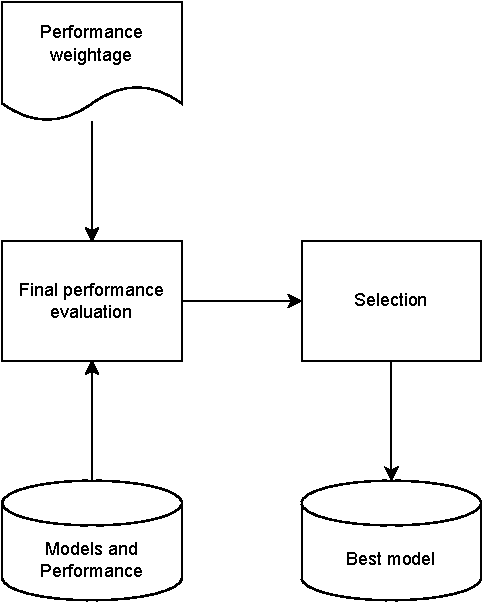
\includegraphics[width=0.6\columnwidth]{media/sec03/selection.pdf}
    \caption{Selection Process}
    \label{fig:selection_process}
\end{figure}

\subsubsection{Prediction Process}\label{subsubsec:prediction_process}

The prediction process is the final process in the system. \autoref{fig:prediction_process}, shows the structure of the prediction process. This process unpacks the best model and loads it for prediction. The model generates predictions with user-provided data. The output is displayed to the user. This output is also stored for future reference.

\begin{figure}[ht]
    \centering
    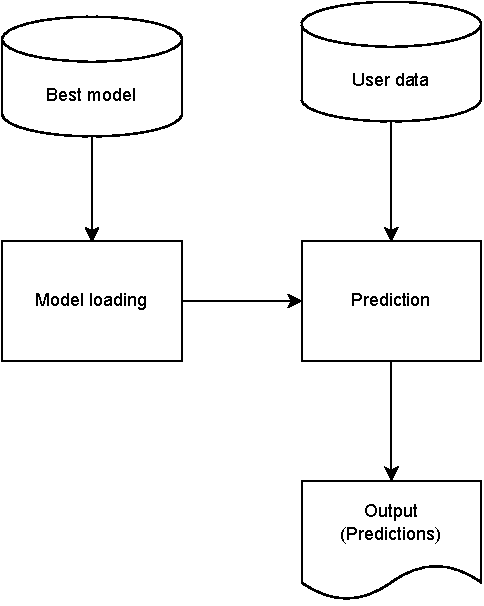
\includegraphics[width=0.6\columnwidth]{media/sec03/prediction.pdf}
    \caption{Prediction Process}
    \label{fig:prediction_process}
\end{figure}

\subsection{Algorithms}\label{subsec:algorithms}

The system uses two algorithms to run. These algorithms are training and selection algorithms and prediction algorithms.

\vspace{-0.5em}
\subsubsection*{Training and Selection Algorithm}\label{subsubsec:training_and_selection_algorithm}
\vspace{0.5em}
\begin{enumerate}
    \item Collect/Receive dataset.
    \item Split data into 80:20 ratio for training and testing.
    \item Build a model from presets.
    \item Train models with training dataset and store models.
    \item Evaluate the performance of models with the testing dataset.
    \item Rank models with help of performance and premade tuning parameters.
    \item Selects the best model and stores it for future use.
\end{enumerate}

\vspace{-0.5em}
\subsubsection*{Prediction Algorithm}\label{subsubsec:prediction_algorithm}
\vspace{0.5em}
\begin{enumerate}
    \item Collect/Receive dataset.
    \item Load best-suited model data from the storage.
    \item Unpack model for predictions.
    \item Make predictions with the provided dataset and loaded model.
    \item Return predictions to user.
\end{enumerate}

\subsection{Implmentation}\label{subsec:implmentation}

\subsubsection{Web Architecture}\label{subsubsec:web_architecture}

The system provides service with a web application. The users aren't allowed to interact with the system directly. This provision is to provide security and reduce the outside influence on results. The interface layer is used for a user to interact with the system indirectly. \autoref{fig:web_architecture}, shows the web architecture of the system. The system is connected to the database directly. A direct connection is provided to access live data. User-provided data is processed by the system and stored in the database.

\begin{figure}[ht]
    \centering
    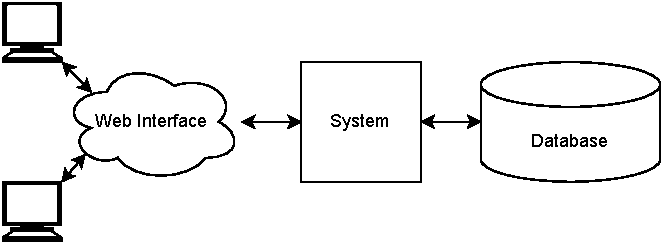
\includegraphics[width=0.9\columnwidth]{media/sec03/web_architecture.pdf}
    \caption{Web Architecture}
    \label{fig:web_architecture}
\end{figure}

\subsubsection*{Web Interface}\label{subsubsec:web_interface}
The web interface provides users with a way to interact with the system. The primary function of the web interface is to provide secure access to the system process. Approved users can interact with various modules on the system. This interface allows users to access selection and prediction processes. Users can upload data to the system.

The interface presents prediction results as well as performance evaluation results. Prediction results are provided in tabular format and stored in CSV files for future reference. Performance results are presented in graphical format and also stored in CSV files for future reference.

\section{Result and Analysis}\label{sec:result_and_analysis}

\subsection{Dataset}\label{subsec:dataset}

% To test the selection system, we used three datasets. All three datasets have very different structures. Dataset 1 [\citenum{sakar2019comparative,parkinsons_disease_classification}] contains 149 records with 23 features. Dataset 2 [\citenum{little2007exploiting,parkinsons_disease_detection}] contains 201 records with 754 features. Dataset 3 [\citenum{ecg_heartbeat}] contains 65661 records with 188 features.

% To test the selection system, we used three datasets. All three datasets have very different structures. Dataset 1 contains 149 records with 23 features [\citenum{parkinsons_disease_classification}]. Dataset 2 contains 201 records with 754 features [\citenum{parkinsons_disease_detection}]. Dataset 3 contains 65661 records with 188 features [\citenum{ecg_heartbeat}].

To test the selection system, we used three datasets. All three datasets have very different structures. Dataset 1 contains 149 records with 23 features [\citenum{parkinsons_disease_classification}]. Dataset 2 contains 201 records with 754 features [\citenum{parkinsons_disease_detection}]. Dataset 3 contains 65661 records with 188 features [\citenum{ecg_heartbeat}].

Dataset 1 is the smallest dataset with a lower number of features compared to other two datasets. Dataset 2 also contains few records, but contains the highest amount of features compared to other two datasets. While, dataset 3 has a large number of records and moderate amount of features.

\subsection{Results}\label{subsec:results}

After providing the datasets mentioned in the previous section, the system trained a few models on those datasets. The application selected the best-suited model based on datasets. 

\autoref{fig:performance_analysis_dataset_1}, shows the performance of various models trained on dataset 1. Due to the small number of records and few features model is overtrained in the case of few models. The values in \autoref{tab:performance_analysis_dataset_1}, suggest that KNN and RF models were overtrained. The KNN model is selected as the best model for this dataset.

\begin{figure}[ht]
    \centering
    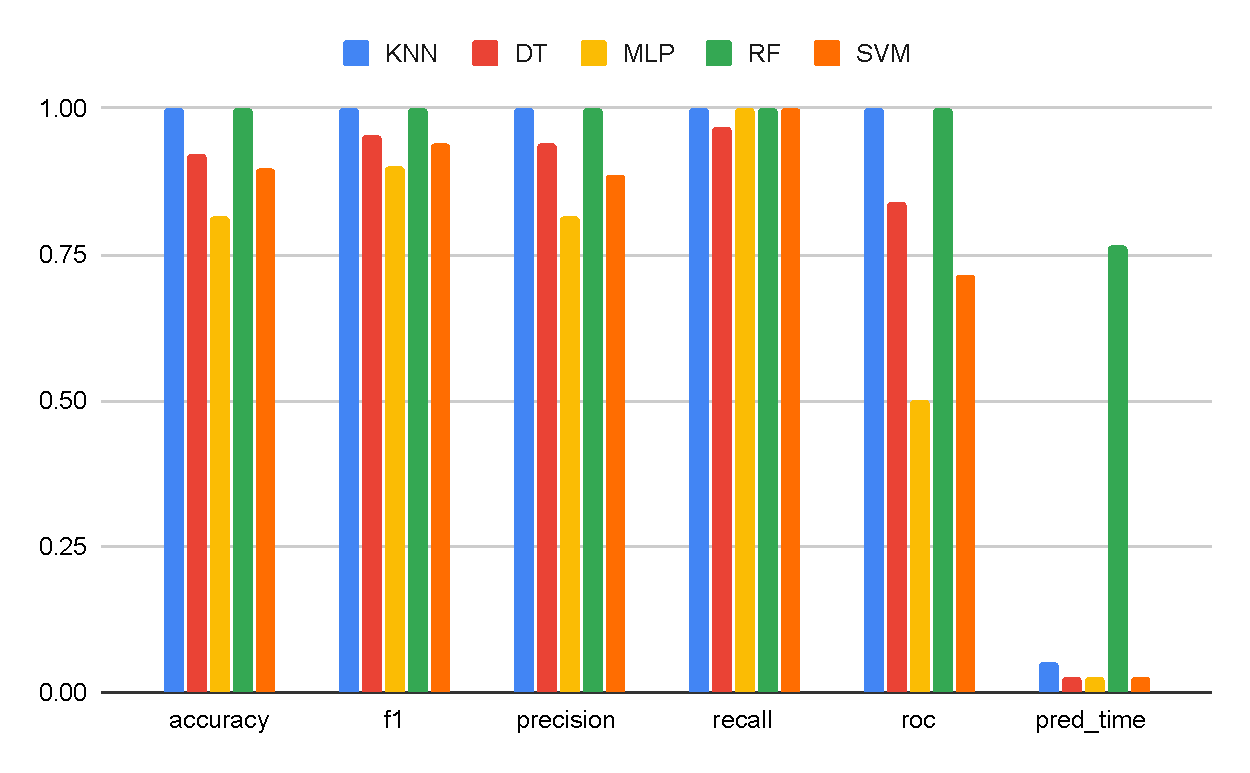
\includegraphics[width=0.9\columnwidth]{media/sec04/dataset_1_performance_evaluation.pdf}
    \caption{Performance Analysis Dataset 1}
    \label{fig:performance_analysis_dataset_1}
\end{figure}

\begin{table}[ht]
\caption{Performance Analysis of Dataset 1}\label{tab:performance_analysis_dataset_1}
\begin{tabular*}{\tblwidth}{@{}LLLLLL@{}}
\toprule
Metrics & KNN & DT & MLP & RF & SVM \\ % Table header row
\midrule
Accuracy & 1.00 & 0.92 & 0.82 & 1.00 & 0.89 \\
F1 & 1.00 & 0.95 & 0.89 & 1.00 & 0.94 \\
Pricision & 1.00 & 0.93 & 0.82 & 1.00 & 0.88 \\
Recall & 1.00 & 0.97 & 1.00 & 1.00 & 1.00 \\
ROC & 1.00 & 0.84 & 0.50 & 1.00 & 0.71 \\
Time & 0.05 & 0.02 & 0.02 & 0.76 & 0.02 \\
\bottomrule
\end{tabular*}
\end{table}

\autoref{fig:performance_analysis_dataset_2}, shows the performance of various models trained on dataset 2. This dataset also had a small number of records, but the number of features is extremely high. The values from \autoref{tab:performance_analysis_dataset_2}, shows the random forest performed better across all parameters but prediction time. The system selected the Random Forest model as best suited mode.

\begin{figure}[ht]
    \centering
    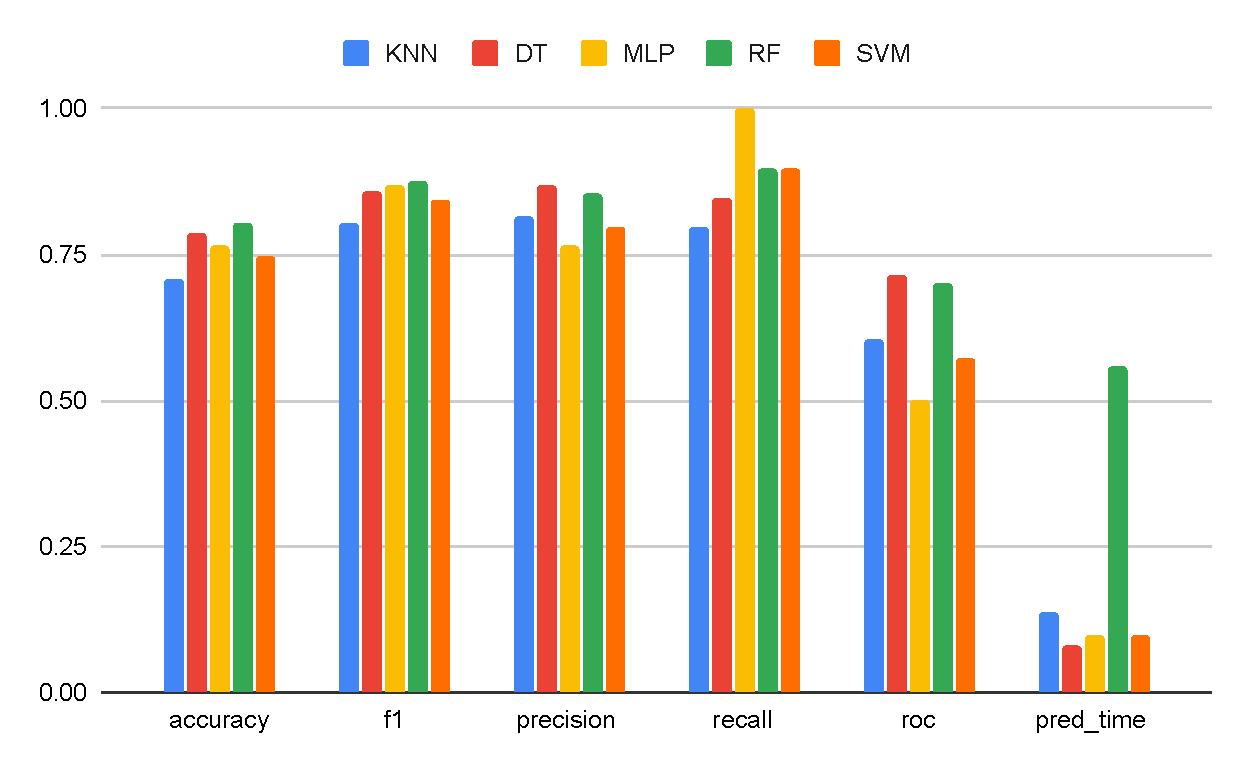
\includegraphics[width=0.9\columnwidth]{media/sec04/dataset_2_performance_evaluation.pdf}
    \caption{Performance Analysis Dataset 2}
    \label{fig:performance_analysis_dataset_2}
\end{figure}

\begin{table}[ht]
\caption{Performance Analysis of Dataset 2}\label{tab:performance_analysis_dataset_2}
\begin{tabular*}{\tblwidth}{@{}LLLLLL@{}}
\toprule
Metrics & KNN & DT & MLP & RF & SVM \\ % Table header row
\midrule
Accuracy & 0.71 & 0.78 & 0.76 & 0.80 & 0.75 \\
F1 & 0.81 & 0.86 & 0.87 & 0.88 & 0.84 \\
Precision & 0.82 & 0.67 & 0.76 & 0.85 & 0.80 \\
Recall & 0.79 & 0.85 & 1.00 & 0.90 & 0.90 \\
ROC & 0.61 & 0.71 & 0.50 & 0.70 & 0.57 \\
Time & 0.13 & 0.07 & 0.09 & 0.55 & 0.09 \\
\bottomrule
\end{tabular*}
\end{table}

\autoref{fig:performance_analysis_dataset_3}, shows the performance of various models trained on dataset 3. This dataset had a very high number of records and a moderate amount of features. The values from \autoref{fig:performance_analysis_dataset_3}, shows that almost all models performed satisfactorily on this dataset. The system selected the SVM model as best suited mode.

\begin{figure}[ht]
    \centering
    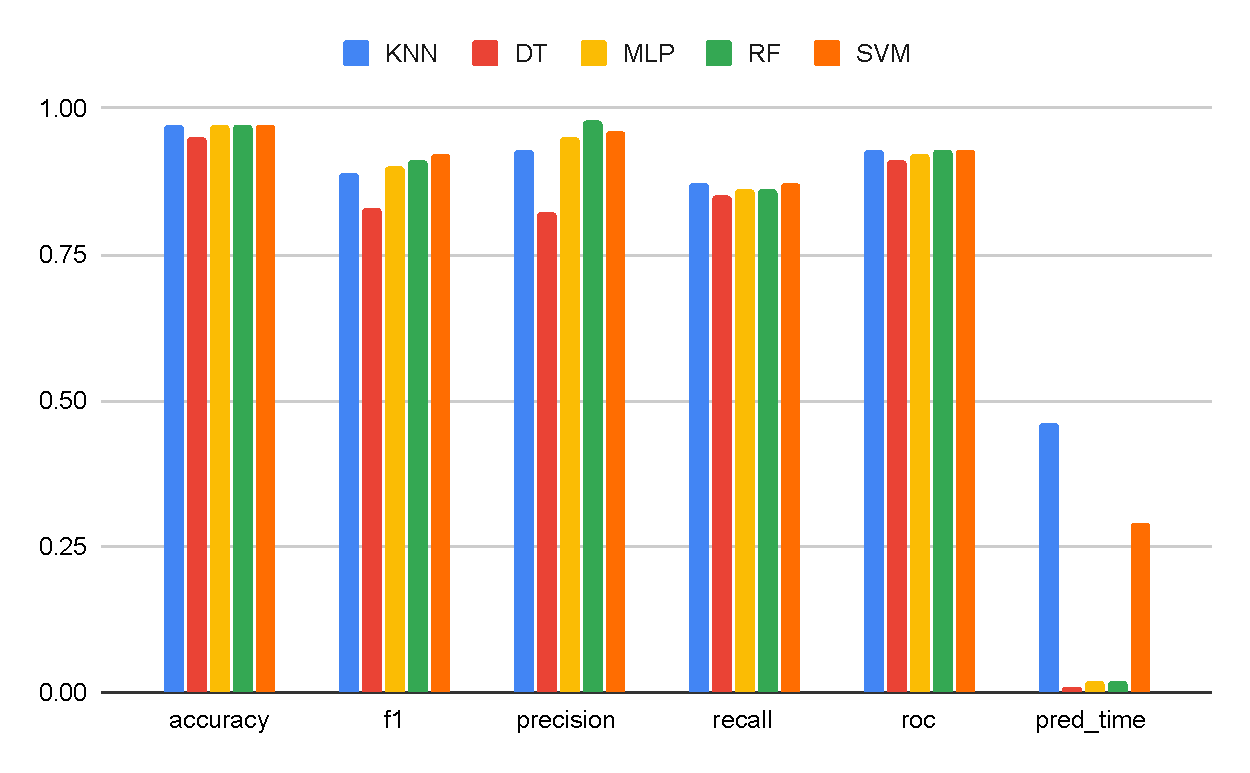
\includegraphics[width=0.9\columnwidth]{media/sec04/dataset_3_performance_evaluation.pdf}
    \caption{Performance Analysis Dataset 3}
    \label{fig:performance_analysis_dataset_3}
\end{figure}

\begin{table}[ht]
\caption{Performance Analysis of Dataset 3}\label{tab:performance_analysis_dataset_3}
\begin{tabular*}{\tblwidth}{@{}LLLLLL@{}}
\toprule
Metrics & KNN & DT & MLP & RF & SVM \\ % Table header row
\midrule
Accuracy & 0.97 & 0.95 & 0.97 & 0.97 & 0.97 \\
F1 & 0.89 & 0.83 & 0.90 & 0.91 & 0.92 \\
Precision & 0.93 & 0.82 & 0.95 & 0.98 & 0.96 \\
Recall & 0.87 & 0.85 & 0.86 & 0.86 & 0.87 \\
ROC & 0.93 & 0.91 & 0.92 & 0.93 & 0.93 \\
Time & 0.46 & 0.01 & 0.02 & 0.02 & 0.29 \\
\bottomrule
\end{tabular*}
\end{table}

\subsection{Key Findings}\label{subsec:key_findings}
From the data displayed in previous section, we saw how the system works on different datasets. These are a few key findings we obtained from that knowledge.
\begin{enumerate}
    \item The system successfully works on different scales of data.
    \item Systems performance does not depends on the number of records.
    \item Systems performance is dependent on the number of features of a dataset.
    \item The system is prone to overfitting depending on the scale of the dataset. Specifically, KNN and RF models tend to overfit with the small scale of data.
    \item The system successfully uses the tuning parameters to select the most suited model from the dataset.
\end{enumerate}

\subsection{Benefits of the System}\label{subsec:benefits_of_system}

The system can be used for any scale of data. It allows users with limited prior knowledge easier access to machine learning technology. As seen in previous section, the system can train multiple models effectively.

The user-defined fine-tuning parameters lead to the selection of the best-suited model for particular tasks. This model can be used to generate predictions in the case of similar datasets. The performance of all models is stored for future evaluation of the system.

\subsection{Improvements On the System}\label{subsec:improvements_on_system}

Currently, the system is limited to only five machine learning algorithms. With the smaller scale of data, specifically with a small number of features, the system tends to overfit the models.  Allowing users to implement their model templates will solve both of these problems.

These algorithms are supervised learning algorithms. The supervised nature of these algorithms limits the training dataset to the labeled dataset. By providing support to unsupervised learning algorithms, systems can accommodate various types of training datasets.

The selection parameters are adjusted before the training process. These predefined parameters restrict the selection choices of the system. Allowing users to tweak selection parameters can increase systems choices.

\section{Conclusion and Future Work}\label{sec:conclusion_and_futur_work}

The system performed satisfactorily during the tests. The application was able to select the model for the provided dataset. The best-suited model showed great accuracy during the prediction process. The whole process required minimum human interaction.

Future work focuses on the implementation of unsupervised learning algorithms. With this, the system will be able to use unlabeled datasets for training. Implementation of continuous learning will be another focus. This will massively increase the adaptability and efficiency of the system.


% Numbered list
% Use the style of numbering in square brackets.
% If nothing is used, default style will be taken.
%\begin{enumerate}[a)]
%\item 
%\item 
%\item 
%\end{enumerate}  

% Unnumbered list
%\begin{itemize}
%\item 
%\item 
%\item 
%\end{itemize}  

% Description list
%\begin{description}
%\item[]
%\item[] 
%\item[] 
%\end{description}  

% Figure
% \begin{figure}[<options>]
% 	\centering
% 		\includegraphics[<options>]{}
% 	  \caption{}\label{fig1}
% \end{figure}


% \begin{table}[<options>]
% \caption{}\label{tbl1}
% \begin{tabular*}{\tblwidth}{@{}LL@{}}
% \toprule
%   &  \\ % Table header row
% \midrule
%  & \\
%  & \\
%  & \\
%  & \\
% \bottomrule
% \end{tabular*}
% \end{table}

% Uncomment and use as the case may be
%\begin{theorem} 
%\end{theorem}

% Uncomment and use as the case may be
%\begin{lemma} 
%\end{lemma}

%% The Appendices part is started with the command \appendix;
%% appendix sections are then done as normal sections
%% \appendix

% \section{}\label{}

\nocite{*}

% To print the credit authorship contribution details
\printcredits

%% Loading bibliography style file
%\bibliographystyle{model1-num-names}
\raggedright
\bibliographystyle{cas-model2-names}

% Loading bibliography database
\bibliography{cas-refs.bib}

% Biography
\bio{}
% Here goes the biography details.
\endbio

% \bio{pic1}
% Here goes the biography details.
\endbio

\end{document}

